%!TEX root = ../main-anran-ma.tex 
% so I can build in this tex file too. 
%************************************************
% \setcounter{theorem}{6}
\chapter{A Proof System}\label{ch:system} % $\mathbb{ZNR}$
%************************************************

We are interested in studying the \define{necessary liberal precondition}, a weakening of the weakest liberal precondition: 
$$wlp.C.F\implies G$$
The weaker $G$ can contain various preconditions: on the one hand, $G$ can be so general that it is satisfied by any program state; on the other hand, a $G$ that is barely weaker than $wlp.C.F$ is also not much different from the latter. 
Alternatively, $G$ can also contain all kinds of preconditions that starting from it, any postcondition is reachable. 
One thing we are certain about, though, is that a program with an original state satisfying $\neg G$ will terminate, and the final state can satisfy $\neg F$: 
\begin{align*}
wlp.C.F\implies G & = \neg G \implies \neg wlp.C.F \\
	& = \neg G \implies wp.C.\neg F 
	\hspace{0.3\textwidth} | \ \todo{insert theorem: wlp and wp are conjugates} 
\end{align*}
In the upcoming sections, we first discuss various forms that the necessary liberal precondition can take and try to identify a $G$ that is most characteristic. 
We proceed then to propose a proof system stemming from the necessary liberal precondition and show its usefulness using an example. \todo{replace with concrete example} 

\section{A Precondition Weaker Than the Weakest Liberal Precondition}
In \autoref{sec:wlp} we defined the weakest liberal precondition and state that it characterizes all the preconditions under whose control the program either \imptt{diverges} or \imptt{will} terminate in a state satisfying $F$. 
We are certain to use ``will'' instead of ``can'', because we view the non-determinism as demonic, so the behavior of wlp can be depicted by \autoref{subfig:wlpd}. 
We can categorize the executions of the program in four ways: 
\begin{enumerate}
	\item the dashed arrow means non-terminating executions; 
	\item the black arrows are executions starting from an initial state satisfying $wlp.C.F$ and only terminating in final states satisfying $F$; 
	\item the green arrows are the executions starting from an initial state satisfying $\neg wlp.C.F$ but can terminate in states either satisfying $F$ or satisfying $\neg F$;
	\item the red arrow represents executions starting from an initial state satisfying $\neg wlp.C.F$ and only terminating in final states satisfying $\neg F$. 
\end{enumerate}

If we were to weaken the precondition, it can happen in various ways as shown in \autoref{subfig:wlp-g-g}{\color{RoyalBlue}-9}. 
We argue that $G$ is most characteristic, when it takes the form as in \autoref{subfig:wlp-g-gg}, because under its control, the program always \imptt{can} reach a final state satisfying $F$ if it terminates, while with an initial state satisfying $\neg G$, the program is \imptt{will} terminate satisfying $\neg F$. 
This behavior is exactly the behavior of wlp, if we were to regard the non-deterministic choice as angelic, as hinted by the similarities between \autoref{subfig:wlp-g-gg} and \autoref{subfig:wp-angelic}. 

\begin{figure}[ht!]\centering
	\subfloat[Weakest liberal precondition (demonic nondeterminism) \label{subfig:wlpd}]{
		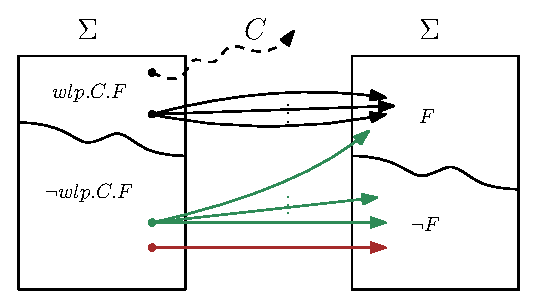
\includegraphics[width=0.4\textwidth]{image/wlp-g/wlpd.eps}
	}
	\hfill

	\subfloat[Precondition $G$ with $wlp.C.F\implies G$ and $G$ contains some green arrows \label{subfig:wlp-g-g}]{
		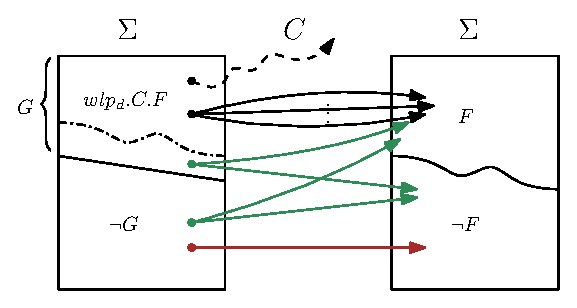
\includegraphics[width=0.45\textwidth]{image/wlp-g/wlp-g-g.eps}
	}
	\hfill
	\subfloat[Precondition $G$ with $wlp.C.F\implies G$ and $G$ contains all the green arrows \label{subfig:wlp-g-gg}]{
		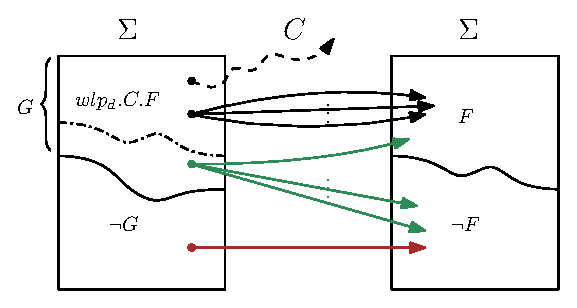
\includegraphics[width=0.45\textwidth]{image/wlp-g/wlp-g-gg.eps}
	}

	\subfloat[Precondition $G$ with $wlp.C.F\implies G$ and $G$ contains some red arrows \label{subfig:wlp-g-r}]{
		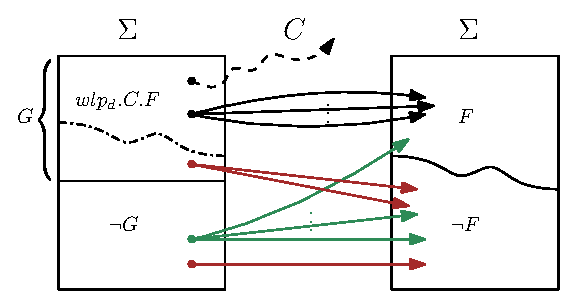
\includegraphics[width=0.45\textwidth]{image/wlp-g/wlp-g-r.eps}
	}
	\hfill
	\subfloat[Precondition $G$ with $wlp.C.F\implies G$ and $G$ contains all the red arrows \label{subfig:wlp-g-rr}]{
		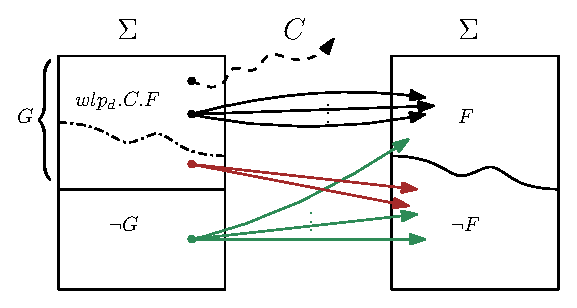
\includegraphics[width=0.45\textwidth]{image/wlp-g/wlp-g-rr.eps}
	}
\caption{Case Distinction of Preconditions Weaker Than wlp (Part 1) }
\label{fig:wlp-g-1}
\end{figure}

\begin{figure}[ht!]\centering
	\ContinuedFloat
	\subfloat[Precondition $G$ with $wlp.C.F\implies G$ and $G$ contains some green arrows and some red arrows \label{subfig:wlp-g-gr}]{
		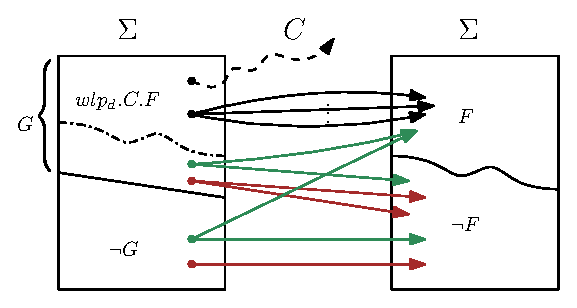
\includegraphics[width=0.45\textwidth]{image/wlp-g/wlp-g-gr.eps}
	}
	\hfill
	\subfloat[Precondition $G$ with $wlp.C.F\implies G$ and $G$ contains all the green arrows and some red arrows \label{subfig:wlp-g-ggr}]{
		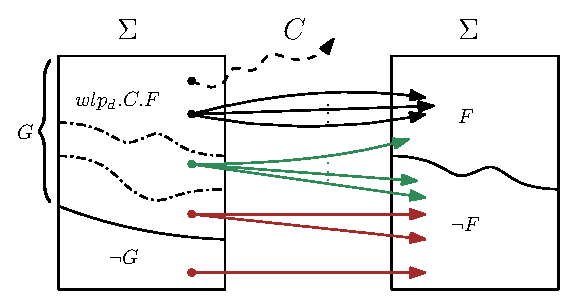
\includegraphics[width=0.45\textwidth]{image/wlp-g/wlp-g-ggr.eps}
	}

	\subfloat[Precondition $G$ with $wlp.C.F\implies G$ and $G$ contains some green arrows and all the red arrows \label{subfig:wlp-g-grr}]{
		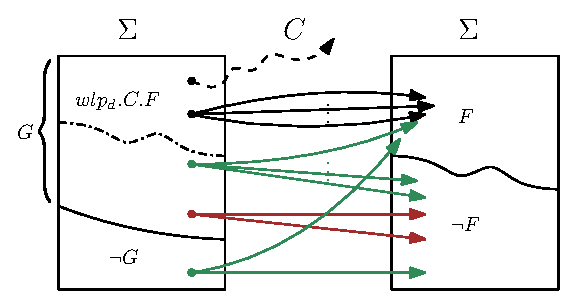
\includegraphics[width=0.45\textwidth]{image/wlp-g/wlp-g-grr.eps}
	}
	\hfill
	\subfloat[Precondition $G$ with $wlp.C.F\implies G$ and $G$ contains all the arrows \label{subfig:wlp-g-ggrr}]{
		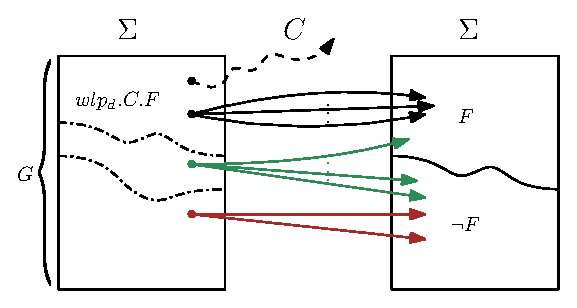
\includegraphics[width=0.45\textwidth]{image/wlp-g/wlp-g-ggrr.eps}
	}
\caption{Case Distinction of Preconditions Weaker Than wlp (Part 2) }
\label{fig:wlp-g-2}
\end{figure}

Dual to the semantics of wp and wlp as shown in \thm{wp-sound} and \thm{wlp-sound}, we can deduce the semantics of wlp with angelic non-determinism (denoted by \define{wlp$_a$}): 
\begin{statement}{wlpa-sound}[Semantics of $wlp_a$]
\ \vspace{-1.5mm}
\[
wlp_a.C.F = \{ \sigma\in\S \mid
\sigma\goto{C}\bot \ \vee\ 
\exists \tau. \sigma\goto{C}\tau:\  \tau\vDash F
 \}
\]
\label{thm:wlpa}
\end{statement}

Luckily, we can find statements using wlp and sp that captures this specific $G$, hence giving us a way to express wlp$_a$ without having to define it: 
\begin{lemma}{wlpa-g}[Angelic wlp implies G]
\ \\ \vspace{-3mm}
	\[\hspace{-2mm}
	\text{ if } \\
	wlp.C.F\implies G
	\\\text{ and } \\ 
	sp.C.\neg G \implies \neg F 
	\\\text{ then } \\ 
	wlp_a.C.F \implies G
	\] 
	\label{lem:wlp-g}
\end{lemma}

\vspace{-1cm}
\begin{proof}
\begin{align*} 
	wlp.C.F\implies G &= \sigma\in wlp.C.F \implies \sigma\in G \\
	& = \sigma\goto{C}\bot\vee \forall \tau.\sigma\goto{C}\tau:\tau\in F \implies \sigma\in G \\
	&\hspace{0.45\textwidth}  \mid \thm{wlp-sound} \\
	& = (\sigma\goto{C}\bot\Longrightarrow \sigma\in G)\vee (\forall \tau.\sigma\goto{C}\tau:\tau\in F \Longrightarrow \sigma\in G) \\
	&\hspace{0.45\textwidth}  \\%\mid \hyperref{(**)}{(**)} \\
	sp.C.\neg G \implies \neg F &= \tau\in sp.C.\neg G \implies \tau\in \neg F \\
	&= \exists \sigma.\sigma\goto{C}\tau:\sigma\in\neg G \implies \tau\in\neg F \\ 
	&\hspace{0.45\textwidth} \mid \thm{sp-sound}\\
	&= \neg (\tau\in\neg F) \implies \neg ( \exists \sigma.\sigma\goto{C}\tau:\sigma\in\neg G ) \\
	&= \tau\in F \implies \forall \sigma.\sigma\goto{C}\tau : \neg (\sigma\in\neg G)\\
	&= \tau\in F \implies \forall \sigma.\sigma\goto{C}\tau : \sigma\in G\\
	wlp_a.C.F \implies G &= \sigma\in wlp_a.C.F \implies \sigma\in G \\
	&= \sigma\goto{C}\bot\vee \exists \tau.\sigma\goto{C}\tau:\tau\in F \implies \sigma\in G \\
	&\hspace{0.45\textwidth} \mid \stm{wlpa-sound}\\
	&= (\sigma\goto{C}\bot\Longrightarrow \sigma\in G )\vee (\exists \tau.\sigma\goto{C}\tau:\tau\in F \Longrightarrow \sigma\in G) \\
yo
\end{align*}

\end{proof}

\begin{lemma}{g-wlpa}[G implies angelic wlp]
\ \\ \vspace{-3mm}
	\[\hspace{-5mm}
	\text{ if } \\
	wlp.C.F\Longrightarrow G
	\\\text{ and } \\ 
	(P\Longrightarrow G) \implies \neg(sp.C.P \Longrightarrow \neg F)
	\text{ then } 
	G \Longrightarrow wlp_a.C.F
	\] 
\end{lemma}

\begin{corollary} [G equivalent to angelic wlp]
	\text{ if } 	$wlp.C.F\Longrightarrow G$
	\  \vspace{-3mm}
	\[\hspace{-6mm}
	\\\text{ and } \\ 
	sp.C.\neg G \Longrightarrow \neg F
	\\\text{ and } \\
	(P\Longrightarrow G) \implies \neg(sp.C.P \Longrightarrow \neg F)
	\\\text{ then } \\ 
	G = wlp_a.C.F
	\] 
\end{corollary}


% bold version of the above lemmas
% \begin{lemma}[Angelic wlp implies G]
% \textbf{If }$wlp.C.F\implies G$\textbf{ and }$sp.C.\neg G \implies \neg F$\textbf{ then }$wlp_a.C.F \implies G$. 
% \end{lemma}

% \begin{lemma}
% \textbf{If }$wlp.C.F\implies G$\textbf{ and }$(P\implies G) \implies \neg(sp.C.P \implies \neg F)$\textbf{ then }$G \implies wlp_a.C.F$. 
% \end{lemma}

% \begin{corollary}
% \textbf{If }$wlp.C.F\implies G$\textbf{ and }$sp.C.\neg G \implies \neg F$ 
% \textbf{ and }$(P\implies G) \implies \neg(sp.C.P \implies \neg F)$
% \textbf{ then }$G = wlp_a.C.F$. 
% \end{corollary}














\newpage
\section{A Proof System}





%*****************************************
%*****************************************
%*****************************************
%*****************************************
%*****************************************
